% File for libamtrack manual
% Copyright 2006, 2010 Steffen Greilich / the libamtrack team
% This file is part of the libAmTrack project (libamtrack.dkfz.org).

\chapter{Introduction}

\la{} is a library of computational routines for the prediction of solid state detector response and radiobiological effectiveness in proton and ion beams. In this field, \la{} focusses on methods that are based on widely used amorphous track models (ATMs) rather than for example microdosimetry models.

Direct comparisons between ATMs are usually hampered by the lack of knowledge on the details of the modelling and computational procedures. We believe that this hinders a wider application of ATMs and the advance towards a better accurracy of their predictions. 

The \la{} project has therefore been started with the intention to provide an open-source, freely available, and comprehensive code for the community. Written in ANSI C, it is designed to be used independent of which platform the user is working on. Furthermore, the idea behind organizing \la{} as a library is that the user can access its functionality from whatever software tools they are using, e.g. MatLab, R, S-Plus etc.

The organization and documentation of the code -- albeit still far from being perfect -- should help to use \la{} for educational purposes as well.


\section{Amorphous track models}

ATMs (in a slightly confusing manner also referred to as 'track structure models') disregard the stochastic energy deposition pattern by secondary electrons around the track of heavy charged particles (protons or ions, HCPs) considering only the averaged dose $d$ as a function of distance $r$ from the trajectory, i.e. the radial dose distribution (Fig. \ref{fig:TST}). 
Their second important assumption is that -- since photons deposit their energy eventually by electrons as well -- local radiation effects are supposed to be the same for photons and HCPs. Thus, the detector response to irradiation with particles of type $T$ and energy $E$ can be predicted from the homogenous bulk photon dose response $S_X(D)$ of the detector system and the spatial deposition of local dose $d(x,y)$ as calculated from the fluences $\Phi(E, T)$ of the particle field. Despite many simplifications, ATMs are reasonably successful in predicting the response for a variety of physical detectors and biological systems \cite{Katz_et_al_1972, Waligorski_and_Katz_1980, Geiss_et_al_1997, Bassler_et_al_2008}. 

\begin{figure*}
	\centering
		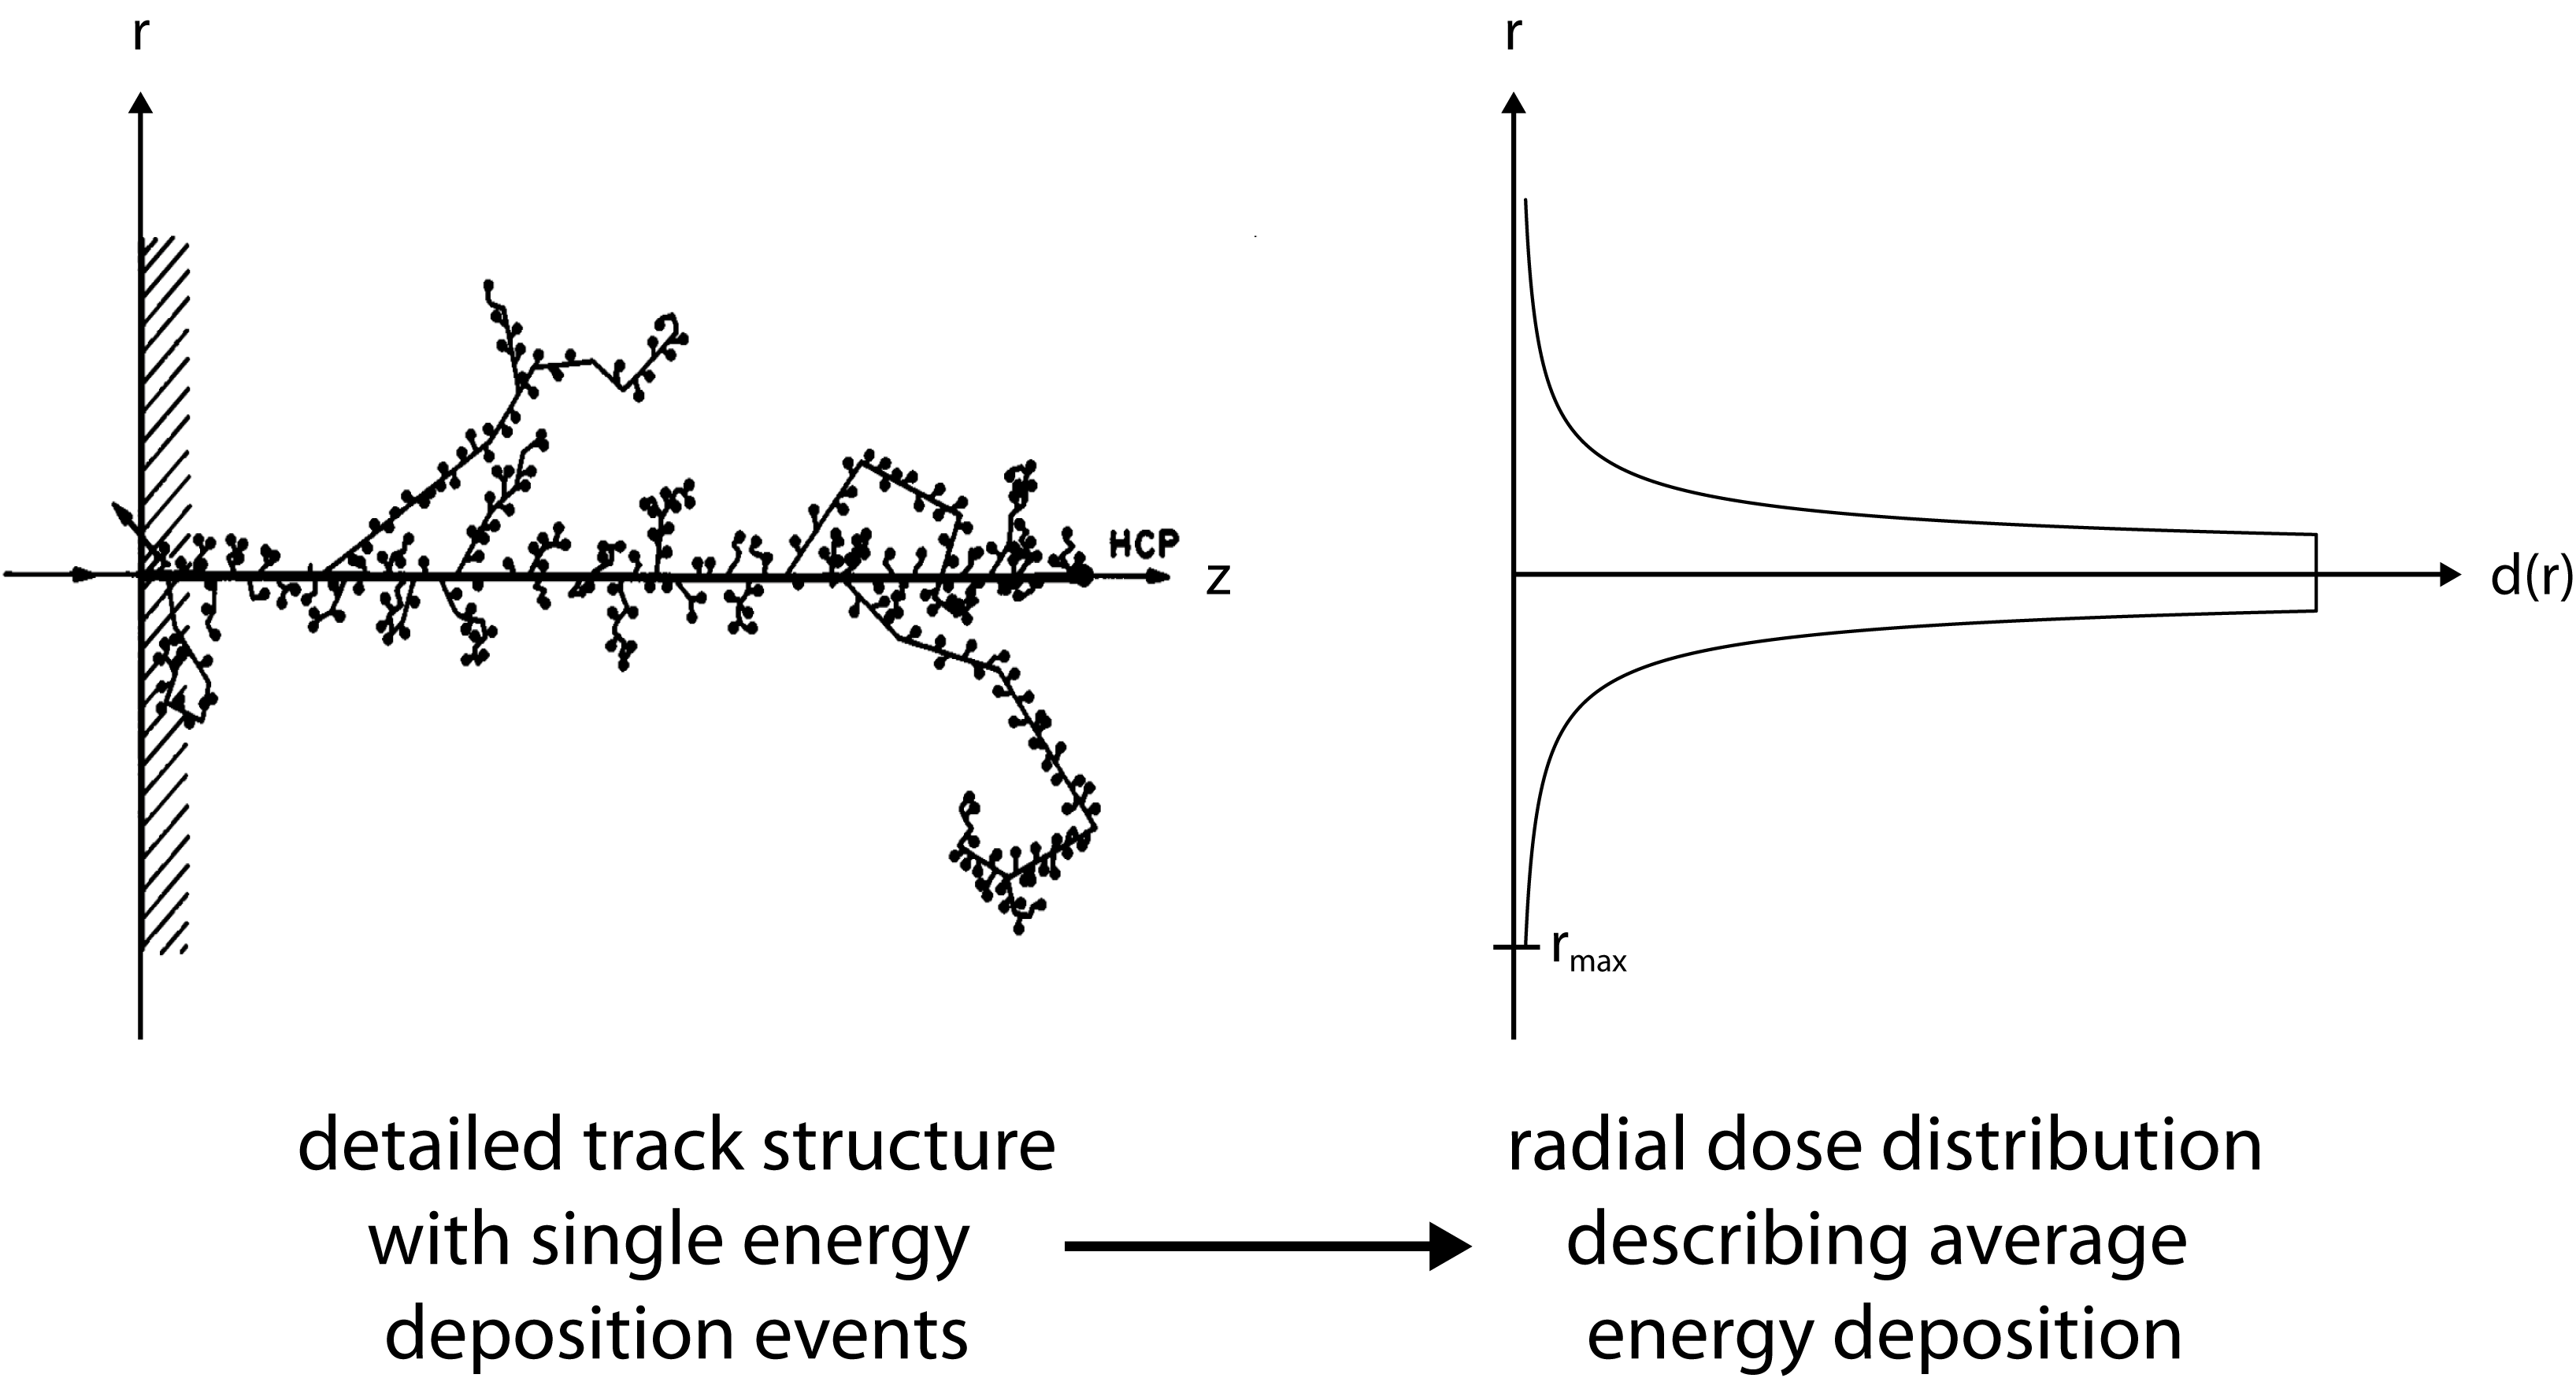
\includegraphics[width=1.0\textwidth]{pictures/TrackStructureDetailAndRDD.png}
	\caption{Amorphization of the detailed track structure.}
	\label{fig:TST}
\end{figure*}


%\section{Microdosimetric models}



\section*{Document status}
\begin{tabular}{l l}
2010.05.28&Created by S. Greilich
\end{tabular}